% Created 2026-05-25 Mon 23:15
\documentclass{article}
\usepackage[utf8]{inputenc}
\usepackage[T1]{fontenc}
\usepackage{graphicx}
\usepackage{longtable}
\usepackage{wrapfig}
\usepackage{rotating}
\usepackage[normalem]{ulem}
\usepackage{amsmath}
\usepackage{amssymb}
\usepackage{capt-of}
\usepackage{hyperref}

\usepackage{fancyhdr}
\usepackage[top=25mm, left=25mm, right=25mm]{geometry}
\usepackage{longtable}
\fancyhead[R]{}
\setlength\headheight{43.0pt}
\usepackage{tabularx}
\usepackage{longtable}
\usepackage[backend=biber, style=ieee]{biblatex}
\addbibresource{/home/evanmh-epn/EPN-Lectures/iccd332ArqComp-2024-B/bibliography/bibliography.bib}
\author{Evan Matango - Edgar Endara - Karen Suaréz - Jose Muela}
\date{26-05-2026}
\title{Taller - Conceptos Básicos de Hardware y Ensamblaje de Computadores\\\medskip
\large ICCD332 Arquitectura de Computadores }
\hypersetup{
 pdfauthor={Evan Matango - Edgar Endara - Karen Suaréz - Jose Muela},
 pdftitle={Taller - Conceptos Básicos de Hardware y Ensamblaje de Computadores},
 pdfkeywords={},
 pdfsubject={},
 pdfcreator={Emacs 29.3 (Org mode 9.6.15)}, 
 pdflang={Spanish}}
\begin{document}

\maketitle
\fancyhead[C]{\includegraphics[scale=0.05]{../images/logoEPN.jpg}\\
ESCUELA POLITECNICA NACIONAL\\FACULTAD DE INGENIERIA DE SISTEMAS\\
ARQUITECTURA DE COMPUTADORES}
\thispagestyle{fancy}


\section{Instrucciones generales}
\label{sec:orgae5fcf4}

Este taller se realiza en \textbf{grupos}. Cada integrante debe completar
individualmente el curso Cisco Networking Academy:
\textbf{Conceptos Básicos de Hardware de Computadora} y obtener su
certificado de completitud. 

\textbf{Entregables del grupo:}
\begin{itemize}
\item Resolución de éste archivo fuente \texttt{.org}
\item El PDF exportado desde Emacs \texttt{M-x org-latex-export-to-pdf}
\item Los certificados individuales de cada integrante (PDF o imagen)
\end{itemize}


\textbf{Entregable Individual(Tarea):}
\begin{itemize}
\item Resolver el cuestionario individual en el aula virtual
\end{itemize}
\subsection{Recursos}
\label{sec:org76bb568}
Cree su usuario en la plataforma de \emph{Cisco Networking Academy}. Use el
siguiente enlace:

\href{https://www.netacad.com/es/courses/computer-hardware-basics?courseLang=en-US}{Cisco Computer Hardware Basics}

Puede configurar según el idioma de su preferencia. El texto está
disponible en Español. Los vídeos disponen de subtítulos en varios
idiomas.

\section{Parte A. Integrantes y certificados}
\label{sec:orgb578b2e}
Para insertar la captura del certificado utilice YASnippet: Escriba
\texttt{fig\_} seguido de \texttt{C-TAB}. Esto produce \texttt{\#+caption}, \texttt{\#+attr\_latex} y
\texttt{\#+label} que permiten colocar un encabezado a la imagen, controlar el
escalado de la misma y una referencia. Finalmente inserte el enlace al
archivo usando \texttt{C-c C-l} o usando
\texttt{[[./carpeta-certificados/cert-int1.pdf]]}
\newpage
\begin{enumerate}
\item \textbf{Integrante 1}
\begin{itemize}
\item \textbf{Nombre completo:} Evan Nicolás Matango Hinostrosa
\item *Correo:*evan.matango@epn.edu,ec
\item \textbf{Certificado adjunto:}  \href{./Certificados/Certificado-evan.pdf}{(Certificado)}
\begin{figure}[htbp]
\centering
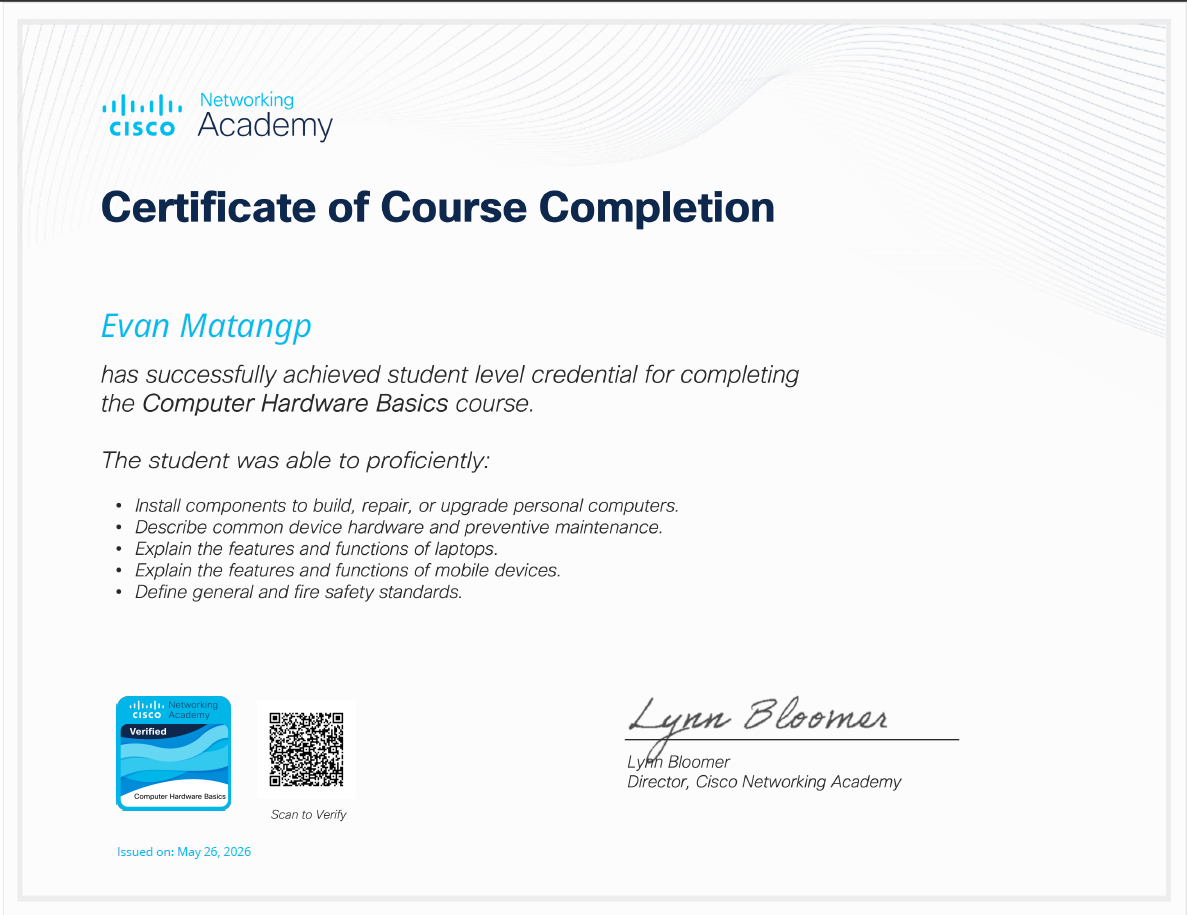
\includegraphics[width=0.75\textwidth]{./Certificados/Certificado-evan.png}
\caption{Certificado de Evan Matango}
\end{figure}

\newpage
\end{itemize}
\item \textbf{Integrante 2}
\begin{itemize}
\item \textbf{Nombre completo:} Endara Roldán Edgar Sebastián
\item \textbf{Correo:} edgar.endara@epn.edu.ec
\item \textbf{Certificado adjunto:}  \href{./Certificados/Certificado-edgar.pdf}{(Certificado)}
\begin{figure}[htbp]
\centering
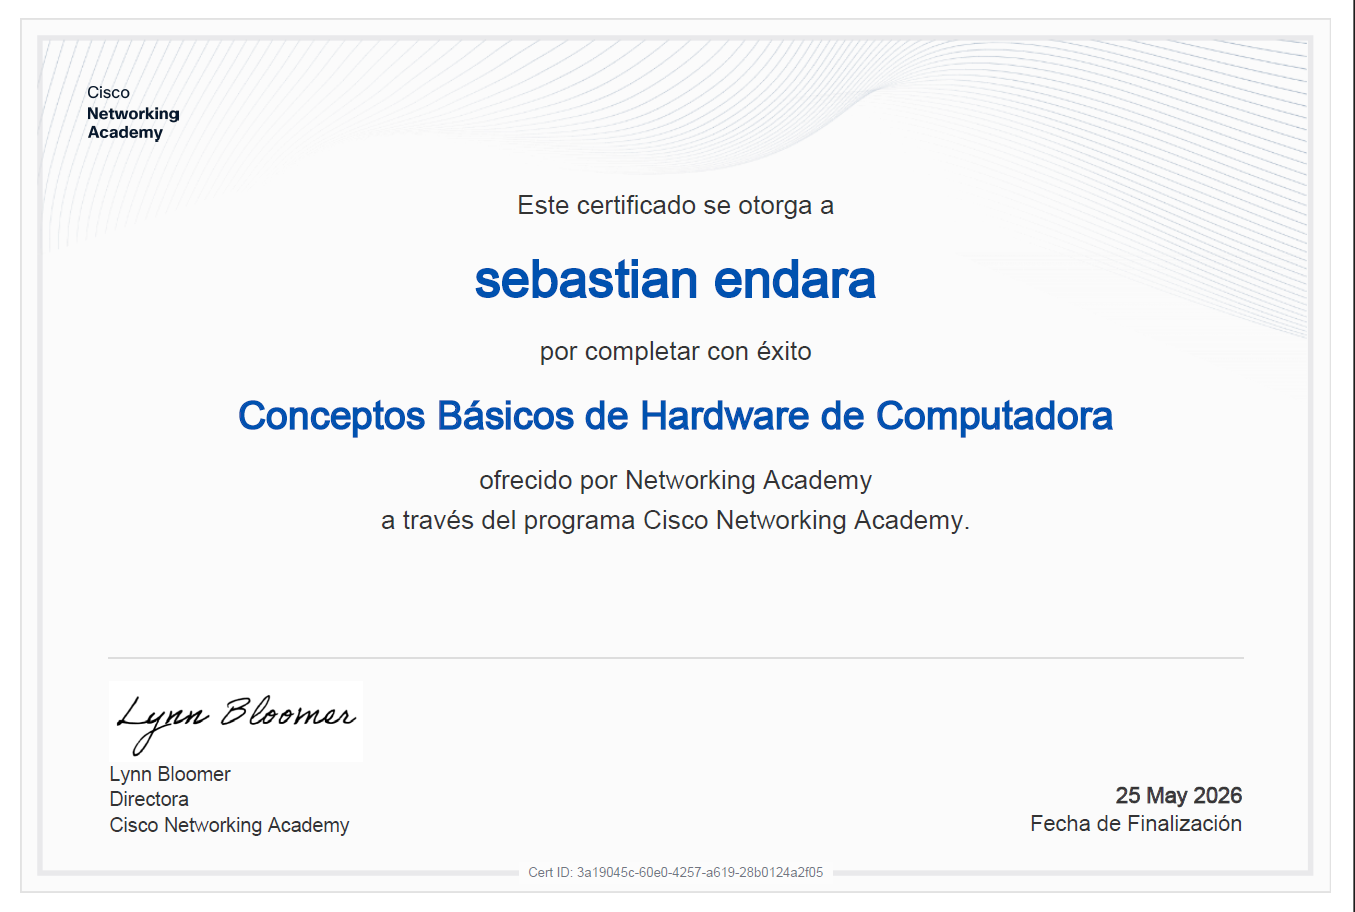
\includegraphics[width=0.75\textwidth]{./Certificados/Certificado-edgar.png}
\caption{Certificado de Edgar Endara}
\end{figure}

\newpage
\end{itemize}
\item \textbf{Integrante 3}
\begin{itemize}
\item \textbf{Nombre completo:} Karen Sofía Suárez Pacheco
\item *Correo:*karen.suarez01@epn.edu.ec
\item \textbf{Certificado adjunto:} \href{./Certificados/Certificado-karen.pdf}{(Certificado)}
\begin{figure}[htbp]
\centering

\includegraphics[width=0.75\textwidth]{./Certificados/Certificado-karen.png}
\caption{Certificado de Karen Suarérz}
\end{figure}
\end{itemize}
\end{enumerate}


\begin{enumerate}
\item \textbf{Integrante 4}
\begin{itemize}
\item \textbf{Nombre completo:} Joset Nicoly Muela Criollo
\item *Correo:*joset.muela@epn.edu.ec
\item \textbf{Certificado adjunto:}
\begin{verbatim}
      Siga las instrucciones para insertar la imagen usando YASnippet
\end{verbatim}
\end{itemize}
\end{enumerate}



\section{Parte B. Cuestionario argumentado grupal}
\label{sec:org40471dd}

Para cada pregunta:

\begin{itemize}
\item Indique la alternativa escogida (letra).
\item Escriba una justificación técnica breve (3 a 6 líneas). Fundamente
su respuesta. Su insumo principal es el curso de Conceptos Básicos
de Hardware. Si usa otro material referenciar.
\item Discuta con el grupo de trabajo las opciones y la respuesta ¿Existió
consenso? ¿Cuáles fueron las principales discrepancias?
\end{itemize}

\textbf{Criterio:} correcto/incorrecto + calidad del argumento técnico.

\subsection{Pregunta 1}
\label{sec:orgb957f47}
Al instalar una CPU en un socket LGA, ¿por qué es crítico alinear el
pin 1 de la CPU con el pin 1 del socket?

a. Para que el sistema arranque con mayor rapidez 

b. Para evitar daños en la CPU y el socket al insertar incorrectamente

c. Porque el pin 1 es el único que conduce electricidad 

d. Para que el disipador quede centrado automáticamente

\begin{itemize}
\item \emph{Alternativa escogida:} b
\item \emph{Justificación técnica:} Es importante alinear el pin 1 de la CPU
con el pin 1 del socket, porque así se coloca en la posición
correcta y si se inserta mal se pueden dañar los contactos del
socket LGA o la CPU, y esto puede causar fallas al encender la
computadora o daños permanentes en el componente.
\item \emph{Debate del grupo:} El grupo estuvo de acuerdo en escoger la alternativa b,
porque la CPU debe colocarse en la posición correcta antes de asegurarla en
el socket, se descartó la opción a porque no mejora la velocidad de arranque,
la opción c porque el pin 1 no es el único que conduce electricidad,
y la opción d porque el disipador se instala después.
\end{itemize}
\subsection{Pregunta 2}
\label{sec:orgf595f5c}
Al montar la placa madre en el gabinete, ¿cuál es la función de los separadores (standoffs)?

a. Sostener el peso de las tarjetas de expansión

b. Evitar cortocircuitos entre la placa madre y el metal del gabinete

c. Mejorar la ventilación de la placa madre

d. Facilitar la alineación del panel de E/S trasero

\begin{itemize}
\item \emph{Alternativa escogida:} b
\item \emph{Justificación técnica:} Los separadores sirven para que la placa
madre no toque directamente el metal del gabinete, porque si la placa madre
hace contacto con el metal puede producirse un cortocircuito y
dañarse algún componente, por eso los separadores ayudan a instalar
la placa de forma segura.
\item \emph{Debate del grupo:} El grupo estuvo de acuerdo en escoger la
alternativa b, porque los separadores evitan el contacto entre la
placa madre y el gabinete, se descartó la opción a porque las
tarjetas se sujetan en sus ranuras, la opción c porque no son para
ventilación, y la opción d porque el panel de E/S se alinea aparte.
\end{itemize}


\subsection{Pregunta 3}
\label{sec:org43622a9}
Según el manual de ensamblaje de Cisco, ¿cuándo NO es necesario aplicar pasta térmica al instalar el disipador sobre la CPU?

a. Cuando la CPU es de alto rendimiento

b. Cuando el disipador ya incluye pasta térmica preaplicada

c. Cuando la CPU tiene más de un año de uso

d. Cuando el gabinete tiene buena ventilación

\begin{itemize}
\item \emph{Alternativa escogida:} [a completar]
\item \emph{Justificación técnica:} [a completar]
\item \emph{Debate del grupo:} [a completar]
\end{itemize}

\subsection{Pregunta 4}
\label{sec:org263f1f5}
¿Por qué se recomienda usar pulsera antiestática y alfombrilla antiestática al manipular componentes internos?

a. Para proteger al técnico de descargas de 220 V

b. Para evitar que la electricidad estática dañe los componentes

c. Para cumplir una norma estética del laboratorio

d. Para que los tornillos no se magneticen

\begin{itemize}
\item \emph{Alternativa escogida:} [a completar]
\item \emph{Justificación técnica:} [a completar]
\item \emph{Debate del grupo:} [a completar]
\end{itemize}
\subsection{Pregunta 5}
\label{sec:org72f7801}
Si al iniciar la computadora por primera vez un LED del panel frontal no funciona, ¿qué indica el manual de Cisco?

a. Reemplazar el conector por uno de repuesto

b. Revisar el BIOS para habilitar el LED

c. Quitar el conector, invertirlo y volver a conectarlo

d. Desconectar y reconectar la fuente de poder

\begin{itemize}
\item \emph{Alternativa escogida:} [a completar]
\item \emph{Justificación técnica:} [a completar]
\item \emph{Debate del grupo:} [a completar]
\end{itemize}

\subsection{Pregunta 6}
\label{sec:orga5ae60d}
¿Por qué una GPU puede requerir un conector de alimentación PCIe adicional de la fuente de poder?

a. Porque la ranura PCIe no transmite señal de video

b. Porque las GPUs de alto rendimiento consumen más potencia de la que la ranura puede suministrar

c. Porque el conector PCIe solo funciona con tarjetas de red

d. Por el estándar de codificación de color de los cables SATA

\begin{itemize}
\item \emph{Alternativa escogida:} [a completar]
\item \emph{Justificación técnica:} [a completar]
\item \emph{Debate del grupo:} [a completar]
\end{itemize}

\section{Parte C. Mantenimiento de computadores}
\label{sec:org76f51c3}

\subsection{3.1 Insumos para mantenimiento preventivo}
\label{sec:org1c10767}
Liste al menos seis insumos y describa para qué sirve cada
uno. Revise el siguiente \href{https://youtu.be/3ri1BMV7XTM?si=bjYoDUUKuMWwj4Qg}{vídeo}.

\begin{center}
\begin{tabular}{ll}
Insumo & Uso principal\\[0pt]
\hline
 & \\[0pt]
 & \\[0pt]
 & \\[0pt]
 & \\[0pt]
 & \\[0pt]
 & \\[0pt]
\end{tabular}
\end{center}

\subsection{3.2 Procedimiento de limpieza — Desktop}
\label{sec:org31818b6}
\begin{enumerate}
\item 

\item 

\item 

\item 

\item 
\end{enumerate}

\subsection{3.3 Procedimiento de limpieza — Laptop}
\label{sec:orgefcb197}
\begin{enumerate}
\item 

\item 

\item 

\item 

\item 
\end{enumerate}

\section{Parte D. Aprendizaje obtenido}
\label{sec:org5aca149}

\subsection{Integrante 1 [Nombre]}
\label{sec:org58ff7f4}
\begin{itemize}
\item \textbf{¿Qué conocimiento nuevo obtuvo del curso?} [Respuesta]
\item \textbf{¿Qué concepto corrigió o clarificó?} [Respuesta]
\end{itemize}

\subsection{Integrante 2 Edgar Endara}
\label{sec:org9c8390f}
\begin{itemize}
\item \textbf{¿Qué conocimiento nuevo obtuvo del curso?} Reforcé mis
conocimientos sobre el ensamblaje de computadoras, ya que tenía
una idea previa sobre armar una PC y limpiar una laptop, pero el
curso me ayudó a entender mejor el orden correcto de instalación
y las medidas para evitar daños físicos o eléctricos.
\item \textbf{¿Qué concepto corrigió o clarificó?} Clarifiqué que los
separadores no solo sostienen la placa madre, también evitan que
toque el metal del gabinete y se produzcan cortocircuitos.
\end{itemize}

\subsection{Integrante 3 [Nombre]}
\label{sec:org966f634}
\begin{itemize}
\item \textbf{¿Qué conocimiento nuevo obtuvo del curso?} [Respuesta]
\item \textbf{¿Qué concepto corrigió o clarificó?} [Respuesta]
\end{itemize}

\subsection{Integrante 3 [Nombre]}
\label{sec:orga131ab5}
\begin{itemize}
\item \textbf{¿Qué conocimiento nuevo obtuvo del curso?} [Respuesta]
\item \textbf{¿Qué concepto corrigió o clarificó?} [Respuesta]
\end{itemize}

\section{Rúbrica de evaluación}
\label{sec:org09374ab}

\begin{center}
\begin{tabular}{lr}
Criterio & Puntaje máximo\\[0pt]
\hline
Certificados individuales completos & 20\\[0pt]
Cuestionario: respuesta correcta (x8) & 30\\[0pt]
Cuestionario: argumento técnico (x8) & 30\\[0pt]
Mantenimiento (tabla + procedimientos) & 20\\[0pt]
TOTAL & 100\\[0pt]
\end{tabular}
\end{center}

\section{¿Cómo referenciar en Emacs?}
\label{sec:orge0473cc}
Para insertar una referencia a un recurso bibliográfico
\begin{enumerate}
\item Puede actualizar el archivo \texttt{../bibliography/bibliography.bib}
\item Escribir en formato \textbf{\textbf{BibTeX}} el recurso bibliográfico
\item Verifique la siguiente configuración al encabezado:
\begin{verbatim}
   #+cite_export: biblatex
   #+LATEX_HEADER: \usepackage[backend=biber, style=ieee]{biblatex}
   #+BIBLIOGRAPHY: ../bibliography/bibliography.bib
\end{verbatim}
\item Usar \texttt{M-x org-cite-insert} para insertar una cita. Aparecerá una
lista. Use los cursores para seleccionar la cita. Ejecute \texttt{C-RET}: \emph{De acuerdo con
\autocite{ledin2022modern}, la arquitectura \ldots{}..}
\item Revise que al final del documento exista \texttt{\#+print\_bibliography:}
\item \textbf{\textbf{Sugerencia:}} Para evitar repetir varias veces el proceso de
exportación, es recomendable cambiar el compilador de \LaTeX a
\texttt{latexmk}. Para esto:
\begin{itemize}
\item \texttt{sudo apt install latexmk}
\item Revise en el encabezado del \texttt{.org} que el compilador escogido sea
\texttt{\#+LATEX\_COMPILER: latexmk}. También puede modificar el archivo
\texttt{init.el} para indicar qué compilador se usa para exportar de
\texttt{.org} a \emph{\LaTeX{}}:
\begin{verbatim}
;; 4.7b Proceso de compilación con latexmk para Org-export
(with-eval-after-load 'ox-latex
  (setq org-latex-pdf-process
        '("latexmk -f -pdf -%latex -interaction=nonstopmode -output-directory=%o %f")))

;; 4.7c Org-cite: biblatex como procesador para exportación LaTeX
(with-eval-after-load 'oc
  (setq org-cite-export-processors
        '((latex biblatex)
          (t basic))))

\end{verbatim}
\end{itemize}
\end{enumerate}
\section{Verificación de Entregables [0\%]:}
\label{sec:org648e27f}
Ejecute \texttt{C-c C-c} sobre los ítems de tarea según se hayan cumplido o
no. Si un ítem no pudo realizarse apunte en la siguiente sección las
razones al respecto.
\begin{itemize}
\item[{$\square$}] Los enlaces a los certificados en el documento \texttt{.org} funcionan.
\item[{$\square$}] Resolución completa del Cuestionario2.
\item[{$\square$}] Revisión del vídeo sobre mantenimiento a computador ASUS.
\item[{$\square$}] Tutorial de Comandos Emacs realizado.
\item[{$\square$}] Lista de insumos para mantenimiento completa.
\item[{$\square$}] Procedimiento de mantenimiento para desktop completo.
\item[{$\square$}] Procedimiento de mantenimiento para laptop completo.
\item[{$\square$}] Revisión de ortografía con \texttt{ispell-buffer} en el buffer
\item[{$\square$}] Generación de Archivo PDF \texttt{M-x org-latex-export-to-pdf}
\item[{$\square$}] Subir al aula virutal archivo \texttt{.org} y \texttt{.pdf}
\end{itemize}

\printbibliography
\end{document}
